% This file was created by matlab2tikz.
%
\definecolor{mycolor1}{rgb}{0.00000,0.44700,0.74100}%
%
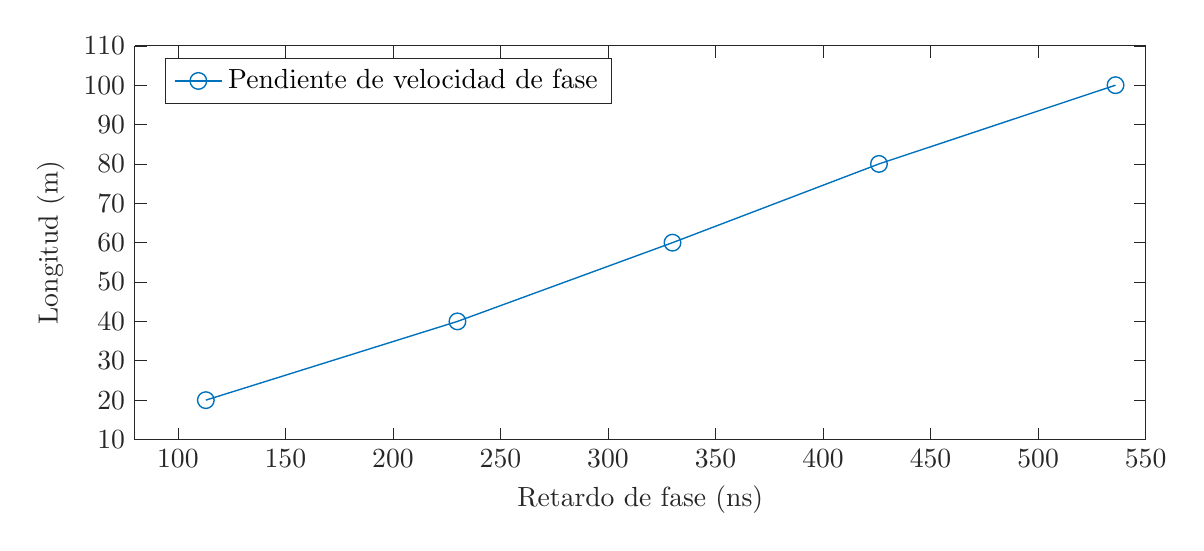
\begin{tikzpicture}

\begin{axis}[%
width=12.837cm,
height=5cm,
at={(0cm,0cm)},
scale only axis,
separate axis lines,
every outer x axis line/.append style={white!15!black},
every x tick label/.append style={font=\color{white!15!black}},
every x tick/.append style={white!15!black},
xmin=80,
xmax=550,
xtick={100,150,200,250,300,350,400,450,500,550},
xlabel style={font=\color{white!15!black}},
xlabel={Retardo de fase (ns)},
every outer y axis line/.append style={white!15!black},
every y tick label/.append style={font=\color{white!15!black}},
every y tick/.append style={white!15!black},
ymin=10,
ymax=110,
ytick={10,20,30,40,50,60,70,80,90,100,110},
ylabel style={font=\color{white!15!black}},
ylabel={Longitud (m)},
axis background/.style={fill=white},
axis on top,
legend style={at={(0.03,0.97)}, anchor=north west, legend cell align=left, align=left, draw=white!15!black}
]
\addplot [color=mycolor1, line width=0.5pt, mark size=3.0pt, mark=o, mark options={solid, mycolor1}]
  table[row sep=crcr]{%
113	20\\
230	40\\
330	60\\
426	80\\
536	100\\
};
\addlegendentry{Pendiente de velocidad de fase}

\end{axis}
\end{tikzpicture}%